\documentclass[aspectratio=169,handout]{beamer}

\makeatletter
\appto\input@path{{pkgs/smile}}
\makeatother

\usetheme[color,german,listings]{tuebix}

\definecolor{blue}{HTML}{26547C}
\definecolor{red}{HTML}{A32638}
\definecolor{green}{HTML}{56AA1C}
\definecolor{black}{HTML}{000000}

\colorlet{smile@lst@color@number}{white}

\usepackage{fontspec}
\setsansfont[
	Path = ./fonts/,
	Scale = 1.2,
	Extension = .ttf,
]{Jersey}
\newfontfamily{\bubbly}[
	Path = ./fonts/,
	Scale = 1,
	Extension = .ttf,
]{04B_30__}

\setbeamerfont{title}{
	size=\huge,
	shape=\bubbly
}

\def\commit#1{\textcolor{blue!40!white}{#1}}

\usepackage{siunitx}
\sisetup{number-mode=match,unit-mode=match,round-mode=places,round-pad=false,group-minimum-digits=4,group-separator=\,}

\usepackage{xfp}
\def\percof#1#2{\num{#1} of \num{#2} (\qty{\fpeval{round(#1*100/#2,2)}}{\percent})}

\usepackage{pgfplots}
\usepackage{pgfplotstable}
\pgfplotsset{
	every axis legend/.append style={style={roundednode}},
	every axis plot/.append style={lw,lcr},
}

\usepackage{emoji}

\usepackage[strict,autostyle]{csquotes}

\def\all{1354928}
\def\merges{101505}
\def\multimerges{2599}

\title{On Cthulu's Merge and Linux's Four Parents}
\author{Lukas Pietzschmann}
\date{Juli 5\textsuperscript{th}, 2025}

\tikzset{
	commit/.style={roundnode,fill=#1},
	commit/.default=white,
	ln/.style={draw,lw,lcr,short=.4mm},
}
\lstset{style=smile@lst@plain}

\begin{document}
\maketitle

\begin{frame}
	\frametitle{Disclaimer}
	\begin{center}
		\LARGE Every number shown here can be reproduced on commit \commit{e60eb44} (v6.15.4)
	\end{center}
\end{frame}

\begin{frame}
	\frametitle{What even is a merge?}
	\begin{columns}[c]
		\begin{column}{0.45\textwidth}
			\begin{itemize}[<+(1)->]
				\item Combine two branches into one additional commit
				\item This is done regularly in the Kernel
				\item \percof{\merges}{\all} commits are merges
				\item But \ldots
			\end{itemize}
		\end{column}
		\begin{column}<2->{0.45\textwidth}
			\scalebox{.8}{\begin{tikzpicture}
				\node[commit=blue!40] (A) {};
				\node[commit=blue!40,right=of A] (B) {};
				\node[commit=blue!40,right=of B] (C) {};
				\node[commit=blue!40,draw=none,fill=none,right=of C] (X) {};
				\node[commit=blue!40,right=of X] (D) {};

				\node[commit=green!25,below=of B] (A2) {};
				\node[commit=green!25,right=of A2] (B2) {};
				\node[commit=green!25,right=of B2] (C2) {};

				\draw[ln] (A) -- (B);
				\draw[ln] (B) -- (C);
				\draw[ln] (C) -- (D);

				\draw[ln] (A2) -- (B2);
				\draw[ln] (B2) -- (C2);

				\draw[ln] (A) to[out=0,in=135] (A2);
				\draw[ln] (C2) to[in=180,out=45] (D);

				\node[shift={(-1cm,1cm)}] at (A) (AL) {\small Base};
				\draw[textarrow] (AL) -- (A);
				\node[shift={(1cm,1cm)}] at (C) (CL) {\small Main tip};
				\draw[textarrow] (CL) -- (C);
				\node[shift={(0cm,-1cm)}] at (C2) (C2L) {\small Feature tip};
				\draw[textarrow] ([yshift=-.6mm]C2L.north) -- (C2);
				\node[shift={(1.5cm,-1cm)}] at (D) (DL) {\small Merge Commit};
				\draw[textarrow] (DL) -- (D);
			\end{tikzpicture}}
		\end{column}
	\end{columns}
\end{frame}

\begin{frame}
	\frametitle{But \ldots}
	\begin{columns}[c]
		\begin{column}{0.6\textwidth}
			\begin{itemize}[<+(1)->]
				\item A merge does not neccessarily only have two parents
				\item \percof{\multimerges}{\merges} merges have more than two parents
				\item We call this an \emph{octopus merge}~\emoji{octopus}
			\end{itemize}
		\end{column}
		\begin{column}<2->{0.3\textwidth}
		\begin{center}
			\scalebox{.8}{\begin{tikzpicture}
				\node[commit=blue!40] (A) {};
				\node[commit=blue!40,right=of A] (B) {};
				\node[commit=blue!40,right=of B] (C) {};
				\node[commit=blue!40,draw=none,fill=none,right=of C] (X) {};
				\node[commit=blue!40,right=of X] (D) {};

				\node[commit=green!25,below=of B] (A2) {};
				\node[commit=green!25,right=of A2] (B2) {};
				\node[commit=green!25,right=of B2] (C2) {};

				\node[commit=red!25,above=of B] (A3) {};
				\node[commit=red!25,right=of A3] (B3) {};
				\node[commit=red!25,right=of B3] (C3) {};

				\node[commit=yellow!25,above=of A3] (A4) {};
				\node[commit=yellow!25,right=of A4] (B4) {};
				\node[commit=yellow!25,right=of B4] (C4) {};

				\draw[ln] (A) -- (B);
				\draw[ln] (B) -- (C);
				\draw[ln] (C) -- (D);

				\draw[ln] (A2) -- (B2);
				\draw[ln] (B2) -- (C2);

				\draw[ln] (A3) -- (B3);
				\draw[ln] (B3) -- (C3);

				\draw[ln] (A4) -- (B4);
				\draw[ln] (B4) -- (C4);

				\draw[ln] (A) to[out=0,in=135] (A2);
				\draw[ln] (C2) to[in=180,out=45] (D);

				\draw[ln] (A) to[out=0,in=215] (A3);
				\draw[ln] (C3) to[in=180,out=-45] (D);

				\draw[ln] (A) to[out=55,in=215] (A4);
				\draw[ln] (C4) to[in=125,out=-45] (D);
			\end{tikzpicture}}
		\end{center}
		\end{column}
	\end{columns}
\end{frame}

\begin{frame}
	\frametitle{How big do they get?}
	\pgfplotsset{width=\textwidth-2cm,height=6cm,compat=1.18}
	\pgfplotstableread[col sep=comma]{merges.csv}\merges
	\begin{tikzpicture}
	\pgfplotstablegetrowsof{\merges}
	\pgfmathtruncatemacro{\rownum}{\pgfplotsretval-1}
	\typeout{\rownum}
	\begin{axis}[axis background/.style={fill=gray!10!black},
		xticklabels from table={\merges}{Parents},
		xtick={0,...,\rownum},
		xlabel=Parents,
		ylabel=Commits (logarithmic),
		yticklabels from table={\merges}{Count},
		ymode=log,log basis y=2,
		axis line style={lw,rnd},
		tick label style={font=\scriptsize},
		ytick={1,6,29,112,761,98907},
		yticklabels={1,6,29,112,761,98907},
	]
		\addplot[ycomb,mark=*,draw=blue,fill=blue!40!black,lw,lcr,rnd] table [x expr=\coordindex, col sep=semicolon, y={Count}] {\merges};
	\end{axis}
	\end{tikzpicture}
	\begin{onlyenv}<2->
		\begin{tikzpicture}[o]
			\clip ([shift={(4.5cm,-2cm)}]current page) circle(1.5cm);
			\node[yshift=6mm] at ([shift={(4.5cm,-2cm)}]current page) {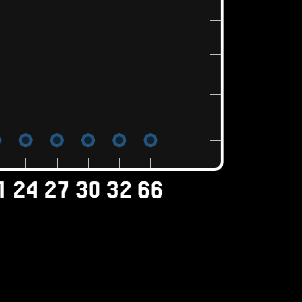
\includegraphics[width=8cm]{66.png}};
			\draw[white,lw] ([shift={(4.5cm,-2cm)}]current page) circle(1.5cm);
		\end{tikzpicture}
	\end{onlyenv}
\end{frame}

\begin{frame}[fragile]
	\tiny\begin{lstlisting}[breakatwhitespace=true,prebreak={}]
commit 2cde51fbd0f310c8a2c5f977e665c0ac3945b46d
Merge: 7471c5c9f58e c097d5fdf3b5 74c375cb85d7 04c3a852f51f 5095f55d7cc3 4f534777c130
       2f54d2a1cf7e 56d37d85438d 192043cf6089 f467a0f513ad bbe580302d33 3990c516de66
       d754fa9ad18d 516ea4b58433 69ae8489076f 25c1a63f43ca f52c91921553 111bd7b18e13
       aafa85e71a75 dd407a324323 71467e46414d 0f7f3d1f17c2 8778ac6be25a 0406a40a095c
       308a0f3f24db 2650bc4f6d0c 8cb7a36eb3a8 323702b4e06d ef749400434c 3cec159cfb3f
       72aa62bed3ea 328089a47112 11db0da831b1 e1771bcf99b0 f60e5473e678 a010ff628c09
       5e8154332f48 58381da68774 626bcacb89f9 38136bde7691 06b2bd23057f 8c5178fca4ce
       8e6ad35a31e7 008ef947d0c5 f58c4fc4a3bf 2309d6757900 5c1537163ce7 b65ab73e5d62
       26090a834b49 9ea6fbc66d15 2c4864334c4d 1769267bb013 f3f9a60f7947 f25cf3496982
       3f3002692ce8 fbbf7fea8e80 c3e8494c001c e40e0b5da87b 50c969732043 63587116811b
       0112b62b12e1 a0a05916cf67 b888edbc68fb d44008b35858 9a199b8e9933 784cbf8ab464
Author: Mark Brown <broonie@linaro.org>
Date:   Thu Jan 2 13:01:55 2014 +0000

Merge remote-tracking branches 'asoc/topic/ad1836', 'asoc/topic/ad193x', 'asoc/topic/adav80x', 'asoc/topic/adsp', 'asoc/topic/ak4641', 'asoc/topic/ak4642', 'asoc/topic/arizona', 'asoc/topic/atmel', 'asoc/topic/au1x', 'asoc/topic/axi', 'asoc/topic/bcm2835', 'asoc/topic/blackfin', 'asoc/topic/cs4271', 'asoc/topic/cs42l52', 'asoc/topic/da7210', 'asoc/topic/davinci', 'asoc/topic/ep93xx', 'asoc/topic/fsl', 'asoc/topic/fsl-mxs', 'asoc/topic/generic', 'asoc/topic/hdmi', 'asoc/topic/jack', 'asoc/topic/jz4740', 'asoc/topic/max98090', 'asoc/topic/mxs', 'asoc/topic/omap', 'asoc/topic/pxa', 'asoc/topic/rcar', 'asoc/topic/s6000', 'asoc/topic/sai', 'asoc/topic/samsung', 'asoc/topic/sgtl5000', 'asoc/topic/spear', 'asoc/topic/ssm2518', 'asoc/topic/ssm2602', 'asoc/topic/tegra', 'asoc/topic/tlv320aic3x', 'asoc/topic/twl6040', 'asoc/topic/txx9', 'asoc/topic/uda1380', 'asoc/topic/width', 'asoc/topic/wm8510', 'asoc/topic/wm8523', 'asoc/topic/wm8580', 'asoc/topic/wm8711', 'asoc/topic/wm8728', 'asoc/topic/wm8731', 'asoc/topic/wm8741', 'asoc/topic/wm8750', 'asoc/topic/wm8753', 'asoc/topic/wm8776', 'asoc/topic/wm8804', 'asoc/topic/wm8900', 'asoc/topic/wm8901', 'asoc/topic/wm8940', 'asoc/topic/wm8962', 'asoc/topic/wm8974', 'asoc/topic/wm8985', 'asoc/topic/wm8988', 'asoc/topic/wm8990', 'asoc/topic/wm8991', 'asoc/topic/wm8994', 'asoc/topic/wm8995', 'asoc/topic/wm9081' and 'asoc/topic/x86' into asoc-next
	\end{lstlisting}
\end{frame}

\begin{frame}
	\frametitle{What \ldots~66 Parents?!}
	Even Linus Torvals himself finds that a bit much:\par\bigskip
	\begin{visibleenv}<2->
	\begin{quote}
		It's pulled, and it's fine, but there's clearly a balance between
		\enquote{octopus merges are fine} and \enquote{Christ, that's not an octopus,
		that's a \textcolor<3->{accent}{Cthulhu merge}}.
	\end{quote}
	\begin{tikzpicture}[o]
		\node[anchor=south east,shift={(-2mm,5mm)}] at (current page.south east) {\color{gray}\tiny\url{https://marc.info/?l=linux-kernel&m=139033182525831}};
	\end{tikzpicture}
	\end{visibleenv}
\end{frame}

\begin{frame}
	\frametitle{How small do they get?}
	\begin{columns}[c]
		\begin{column}{0.5\textwidth}
			\begin{itemize}[<+(1)->]
				\item This also goes the other way around
				\item Let's look at commits with no parents
				\item We call these \emph{init commits}
				\item Let's see \ldots
			\end{itemize}
		\end{column}
		\begin{column}<3->{0.4\textwidth}
			\begin{center}
			\scalebox{.8}{\begin{tikzpicture}
				\node[commit=blue!40] (A) {};
				\node[commit=blue!40,right=of A] (B) {};
				\node[commit=blue!40,right=of B] (C) {};
				\node[commit=blue!40,draw=none,fill=none,right=of C] (X) {};
				\node[commit=blue!40,right=of X] (D) {};

				\node[commit=green!25,below=of B] (A2) {};
				\node[commit=green!25,right=of A2] (B2) {};
				\node[commit=green!25,right=of B2] (C2) {};

				\draw[ln] (A) -- (B);
				\draw[ln] (B) -- (C);
				\draw[ln] (C) -- (D);

				\draw[ln] (A2) -- (B2);
				\draw[ln] (B2) -- (C2);

				\draw[ln] (A) to[out=0,in=135] (A2);
				\draw[ln] (C2) to[in=180,out=45] (D);

				\node[shift={(-1cm,1cm)}] at (A) (AL) {\small Init};
				\draw[textarrow] (AL) -- (A);
			\end{tikzpicture}}
			\end{center}
		\end{column}
	\end{columns}
\end{frame}

\begin{frame}[fragile,t]
	\frametitle{Let's see \ldots}
	\begin{lstlisting}
		git log --max-parents=0 --oneline
	\end{lstlisting}\pause
	\begin{lstlisting}
a101ad945113§\m{h}§ §\color<6->{darkgray!30!black}Share upstreaming patches§
cd26f1bd6bf3§\m{g}§ §\color<5->{darkgray!30!black}greybus: Initial commit§
be0e5c097fc2§\m{b}§ §\color<4->{darkgray!30!black}Btrfs: Initial checkin, basic working tree code§
1da177e4c3f4§\m{l}§ §\color<3->{darkgray!30!black}Linux-2.6.12-rc2§
	\end{lstlisting}
	\begin{tikzpicture}[o]
		\node[shift={(1mm,-1.7mm)},anchor=south west,visible on=<3->] at (pic cs:l) {\scriptsize OG init};
		\node[shift={(1mm,-1.7mm)},anchor=south west,visible on=<4->] at (pic cs:b) {\scriptsize BTRFS init};
		\node[shift={(1mm,-2.1mm)},anchor=south west,visible on=<5->] at (pic cs:g) {\scriptsize GreyBus init};
		\node[shift={(1mm,-1.7mm)},anchor=south west,visible on=<6->] at (pic cs:h) {\scriptsize \emoji{man-shrugging-medium-skin-tone}};
	\end{tikzpicture}
	\begin{itemize}[<+(5)->]
		\item Both BTRFS and GreyBus were developed from a clean project
		\item After merging them, they introduced their respective init commits into the
			kernel
		\item I have no idea wht's up with \commit{a101ad945113}
	\end{itemize}
\end{frame}

\begin{frame}
	\frametitle{Everything Tougether}
	\begin{center}
	\begin{tikzpicture}[node distance=5mm and 15mm,
			commit/.style={roundnode,fill=white,minimum width=15mm,minimum height=15mm},
			commitx/.style={roundnode,fill=lightgray,minimum width=1cm,minimum height=1cm},
			% ln/.style={draw,lw,lcr,short=.4mm,dashed},
		]
		\node[commit] (HEAD) {\color{black}HEAD};

		\node[commit,left=of HEAD] (C) {\color{black}2cde};

		\node[commitx,left=of C] (X) {};

		\node[commit,left=of X,yshift=08mm] (L) {\color{black}1da1};
		\node[commit,left=of X,yshift=-8mm] (B) {\color{black}be0e};
		\node[commit,below=of C] (G) {\color{black}cd26};
		\node[commit,below=of G] (H) {\color{black}a101};

		\draw[ln] (G) to[in=180] (HEAD);
		\draw[ln] (H) to[in=180] (HEAD);

		\draw[ln] (C) to (HEAD);

		\draw[ln] (L) to[out=0,in=180] (X);
		\draw[ln] (B) to[out=0,in=180] (X);

		\foreach\i in {10,20,30,40,50,60,70} {
			\draw[ln] (X) to[bend left=\i] (C);
			\draw[ln] (X) to[bend right=\i] (C);
		}
			\draw[ln] (X) to (C);
	\end{tikzpicture}
	\end{center}
\end{frame}
\end{document}
